\documentclass[11pt]{article}
\usepackage[margin=1in]{geometry}
\usepackage{graphicx}
\usepackage{amsmath, amssymb}
\usepackage{booktabs}
\usepackage{hyperref}
\usepackage{subcaption}

\title{Clustering Method Exploration for Transition State Geometries\\[0.3em]
\large Isopropanol on DFTB0 --- 74 TS, 131 Methods Tested}
\author{Memo \"Ozdincer}
\date{March 2026}

\graphicspath{{figures/clustering_exploration/}}

\begin{document}
\maketitle

\begin{abstract}
We systematically compare 131 clustering configurations across 7 algorithm families
(hierarchical, DBSCAN, OPTICS, KMeans, spectral, agglomerative) applied to 74
transition state geometries of isopropanol on DFTB0.
The distance metric is aligned RMSD (Kabsch + Hungarian).
We evaluate against energy-based ground truth (16 groups), internal quality (silhouette),
and cross-method agreement.
The central finding is that \textbf{RMSD-based structural clustering does not correlate
with energy-based grouping} (all ARI $< 0.05$), meaning structurally similar TS can
have very different energies.
DBSCAN robustly identifies 7 tight structural clusters, but these are not energy-coherent.
\end{abstract}

%----------------------------------------------------------------------
\section{Setup}

\textbf{Data:} 74 converged TS geometries from NR$\to$GAD search on isopropanol (C$_3$H$_8$O, 12 atoms)
at 0.2--0.5~\AA{} noise on the DFTB0 PES. Each TS satisfies $n_{\text{neg}} = 1$ and
$\|F\| < 0.01$~eV/\AA.

\textbf{Distance metric:} Aligned RMSD with Kabsch rotation, Hungarian atom matching
(6 equivalent methyl H), and methyl carbon permutation enumeration.
All 74$\times$74 = 2701 unique pairwise distances precomputed.

\textbf{Ground truth:} Energy-based clusters with 0.1~eV tolerance produce 16 groups.
The 5 main families (A--E) contain 13--17 members each; the remaining 11 groups are singletons or pairs at unique energies.

\textbf{Methods tested:} 131 configurations:
\begin{itemize}
  \item Hierarchical (complete, average, single linkage): thresholds 0.1--0.5~\AA, $k = 3$--20
  \item Hierarchical (Ward): on MDS embedding (Ward requires Euclidean input)
  \item DBSCAN: $\varepsilon = 0.05$--0.5, min\_samples $= 2, 3, 5$
  \item OPTICS: min\_samples $= 2, 3, 5$
  \item KMeans: $k = 3$--20 on MDS embedding
  \item Spectral: $\sigma = $ median and 25th percentile of RMSD, $k = 3$--10
  \item Agglomerative (sklearn): complete/average/single, $k = 3$--10
\end{itemize}

\textbf{Evaluation metrics:}
\begin{itemize}
  \item Adjusted Rand Index (ARI) vs.\ energy clusters
  \item Silhouette score on RMSD matrix
  \item Calinski--Harabasz on MDS embedding
  \item Mean within-cluster energy std (lower = more energy-coherent)
  \item Pairwise ARI between methods (cross-method agreement)
\end{itemize}

%----------------------------------------------------------------------
\section{Structure vs.\ Energy: No Correlation}

\begin{figure}[h]
  \centering
  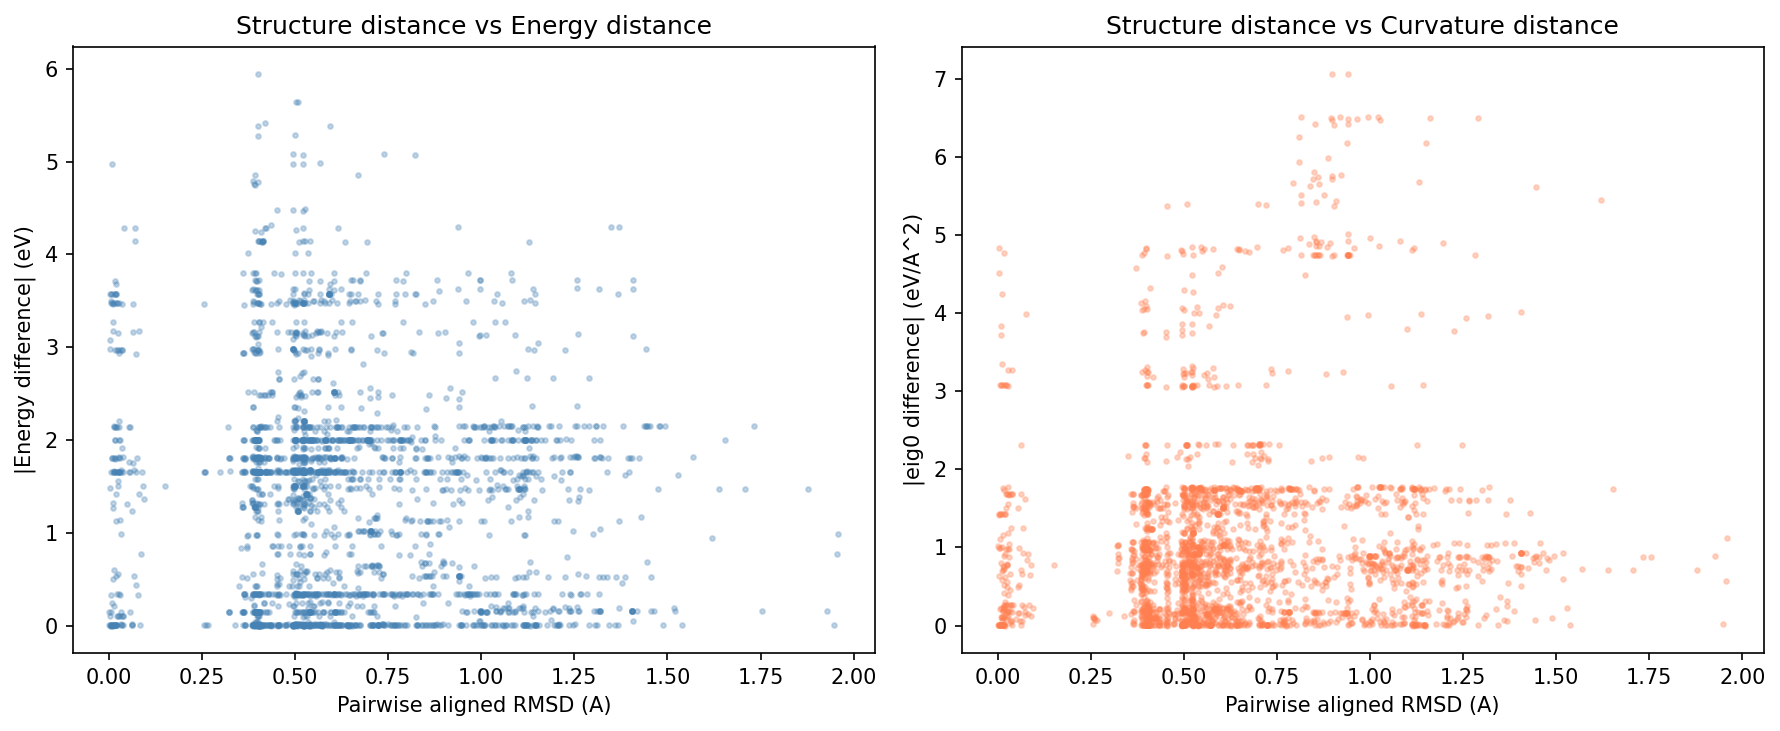
\includegraphics[width=\textwidth]{rmsd_vs_energy_scatter.png}
  \caption{Pairwise aligned RMSD vs.\ energy difference (left) and curvature difference (right)
  for all $\binom{74}{2} = 2701$ TS pairs. There is no correlation: pairs at RMSD $\sim 0.5$~\AA{}
  span 0--6~eV in energy. Curvature (lowest eigenvalue) shows similarly no correlation with structural distance.
  This means RMSD alone cannot distinguish chemically distinct TS families.}
  \label{fig:scatter}
\end{figure}

Figure~\ref{fig:scatter} is the most important result. It shows that \textbf{structural similarity (RMSD)
and chemical identity (energy) are essentially independent} for this molecule and PES.
Two TS with RMSD $= 0.3$~\AA{} (seemingly similar) can differ by 4~eV,
while two TS with RMSD $= 1.0$~\AA{} (seemingly different) can have the same energy.

\begin{figure}[h]
  \centering
  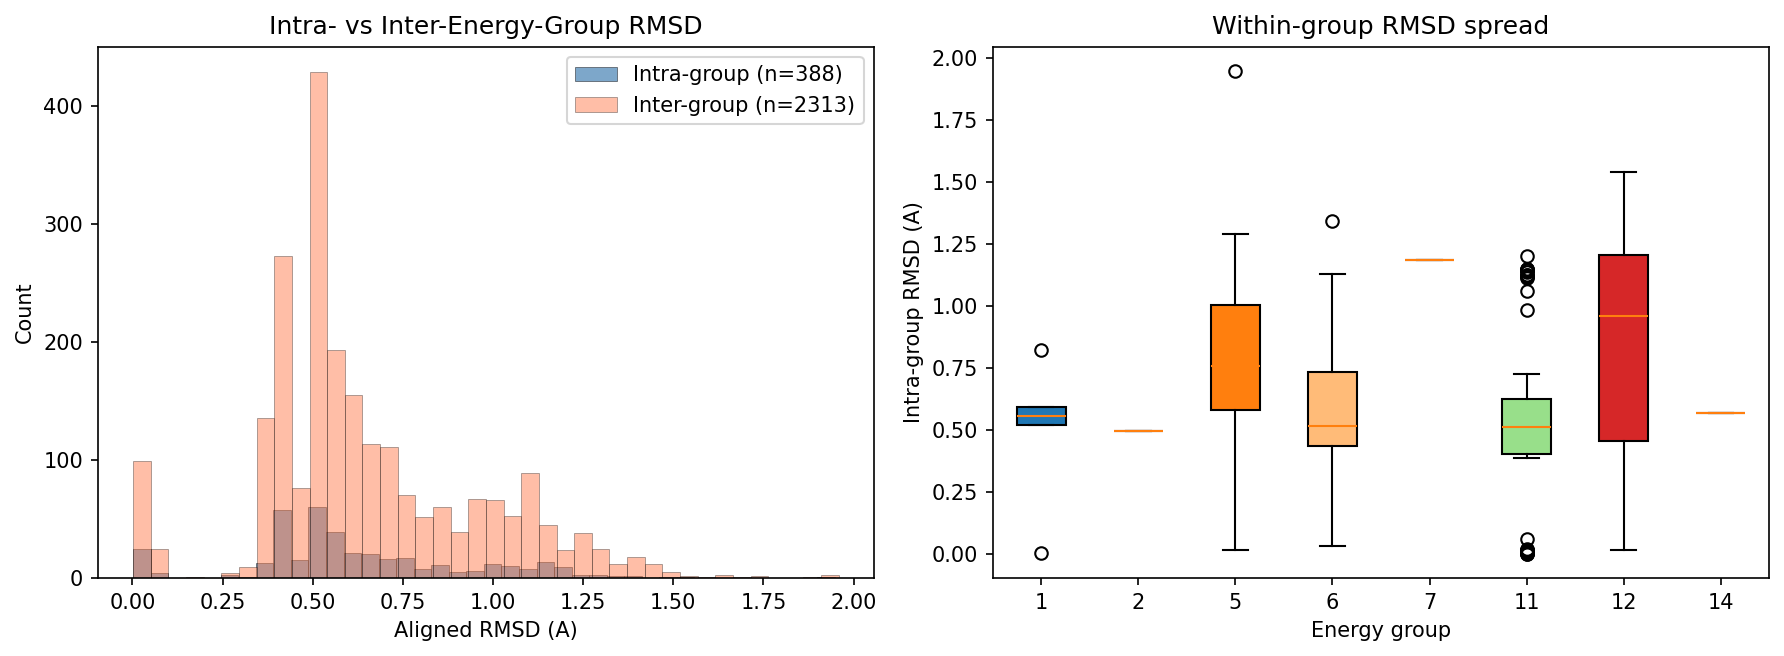
\includegraphics[width=\textwidth]{rmsd_band_analysis.png}
  \caption{Left: distribution of intra-energy-group and inter-energy-group RMSD.
  Heavy overlap: the distributions are not separable, so no RMSD threshold cleanly distinguishes
  same-energy from different-energy TS pairs.
  Right: within-group RMSD spread per energy group. Most groups have 0.3--1.0~\AA{} internal spread.}
  \label{fig:bands}
\end{figure}

Figure~\ref{fig:bands} confirms this quantitatively: intra-group and inter-group RMSD distributions
overlap heavily. The earlier analysis with 67 TS showed a ``natural gap'' at 0.14--0.26~\AA{};
with 74 TS this gap has filled in, suggesting it was a small-sample artifact.

%----------------------------------------------------------------------
\section{Is There a Natural Cluster Count?}

\begin{figure}[h]
  \centering
  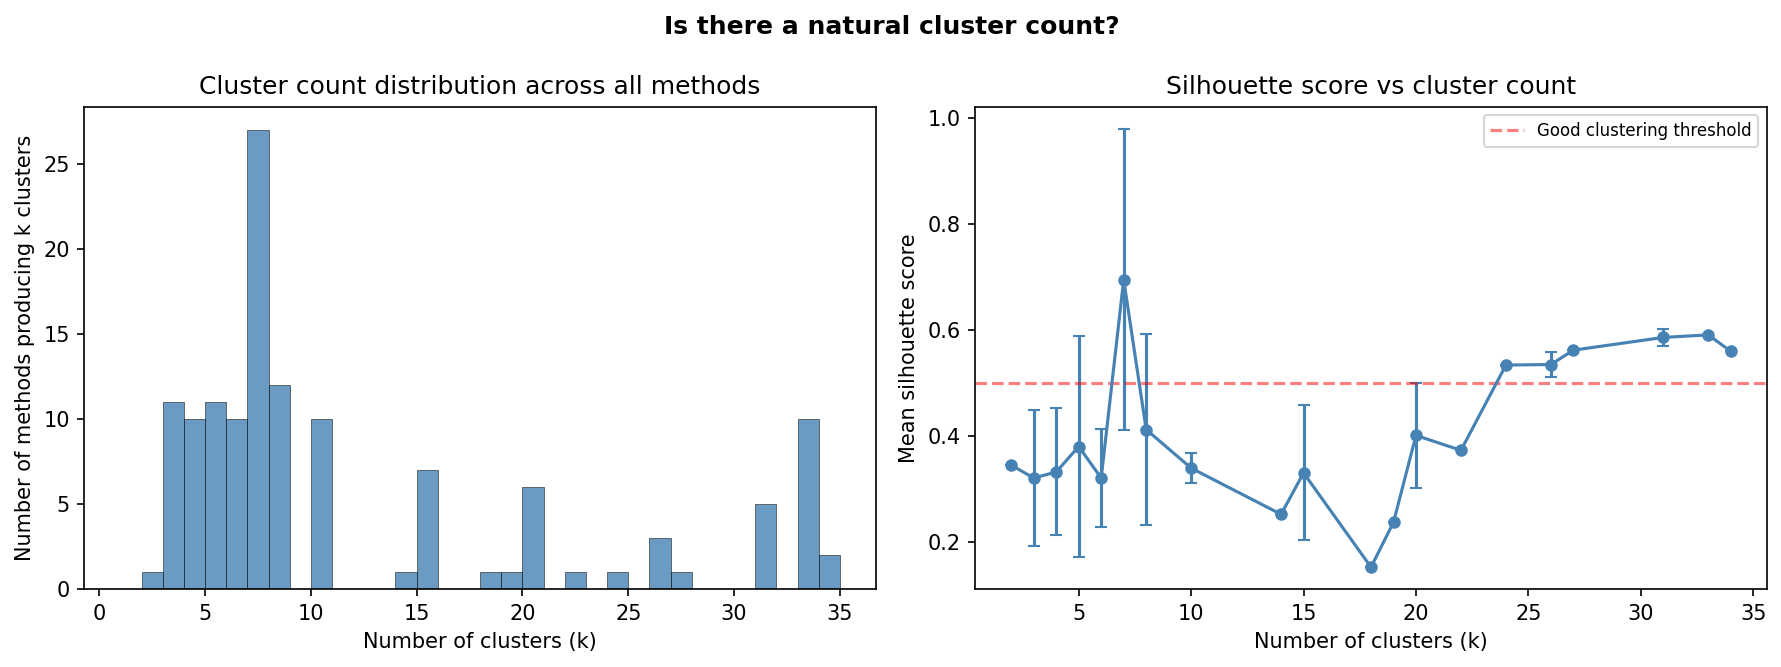
\includegraphics[width=\textwidth]{cluster_count_analysis.png}
  \caption{Left: histogram of cluster counts across all 131 methods. Most methods produce $k = 7$ or
  $k = 31$; no single $k$ dominates.
  Right: silhouette score vs.\ $k$ for hierarchical average linkage. Silhouette is highest at $k = 2$ (trivial split)
  and at high $k$ ($\sim 29$, many singletons). No clear elbow suggests there is no single ``correct'' number of
  structural clusters.}
  \label{fig:kcount}
\end{figure}

The answer is \textbf{no clear natural $k$}. The silhouette curve (Fig.~\ref{fig:kcount}, right) decreases
monotonically from $k = 2$ to $k \approx 15$, then rises again as clusters become singletons.
DBSCAN consistently finds $k = 7$ (for $\varepsilon = 0.05$--0.25), suggesting 7 tight structural
clusters exist, but these account for only 44--48 of 74 TS; the rest are ``noise'' (26--30 points).

%----------------------------------------------------------------------
\section{Cross-Method Agreement}

\begin{figure}[h]
  \centering
  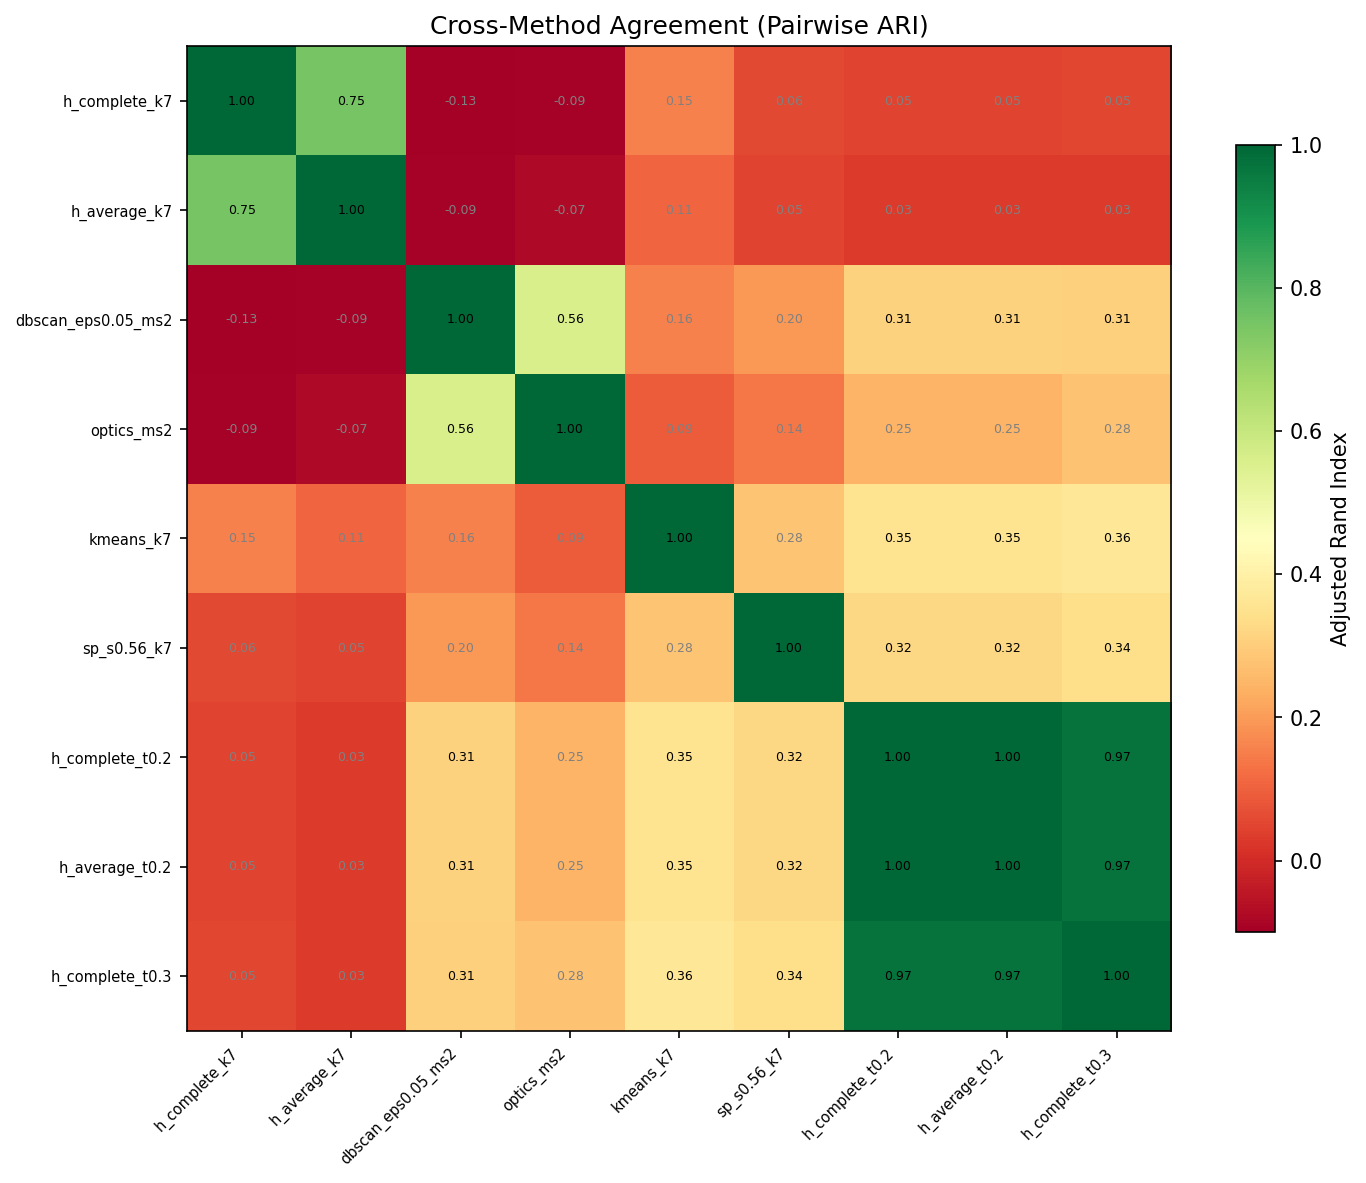
\includegraphics[width=0.75\textwidth]{cross_method_agreement.png}
  \caption{Pairwise ARI between representative methods from each algorithm family.
  Hierarchical complete and average linkage at threshold 0.2~\AA{} agree perfectly (ARI $= 1.0$).
  Hierarchical methods agree moderately with each other (0.3--0.5).
  DBSCAN/OPTICS form their own block (ARI $\sim 0.6$).
  Spectral and KMeans show low agreement with everything ($< 0.2$).
  Overall mean ARI $= 0.25$.}
  \label{fig:agreement}
\end{figure}

Methods \textbf{within} the same family agree reasonably well: hierarchical variants agree at 0.3--1.0
and density-based methods (DBSCAN, OPTICS) agree at $\sim 0.6$.
Methods \textbf{across} families show poor agreement (ARI $< 0.2$).
This means the cluster assignments are method-dependent, not an intrinsic property of the data.

%----------------------------------------------------------------------
\section{Dendrogram with Chemical Features}

\begin{figure}[h]
  \centering
  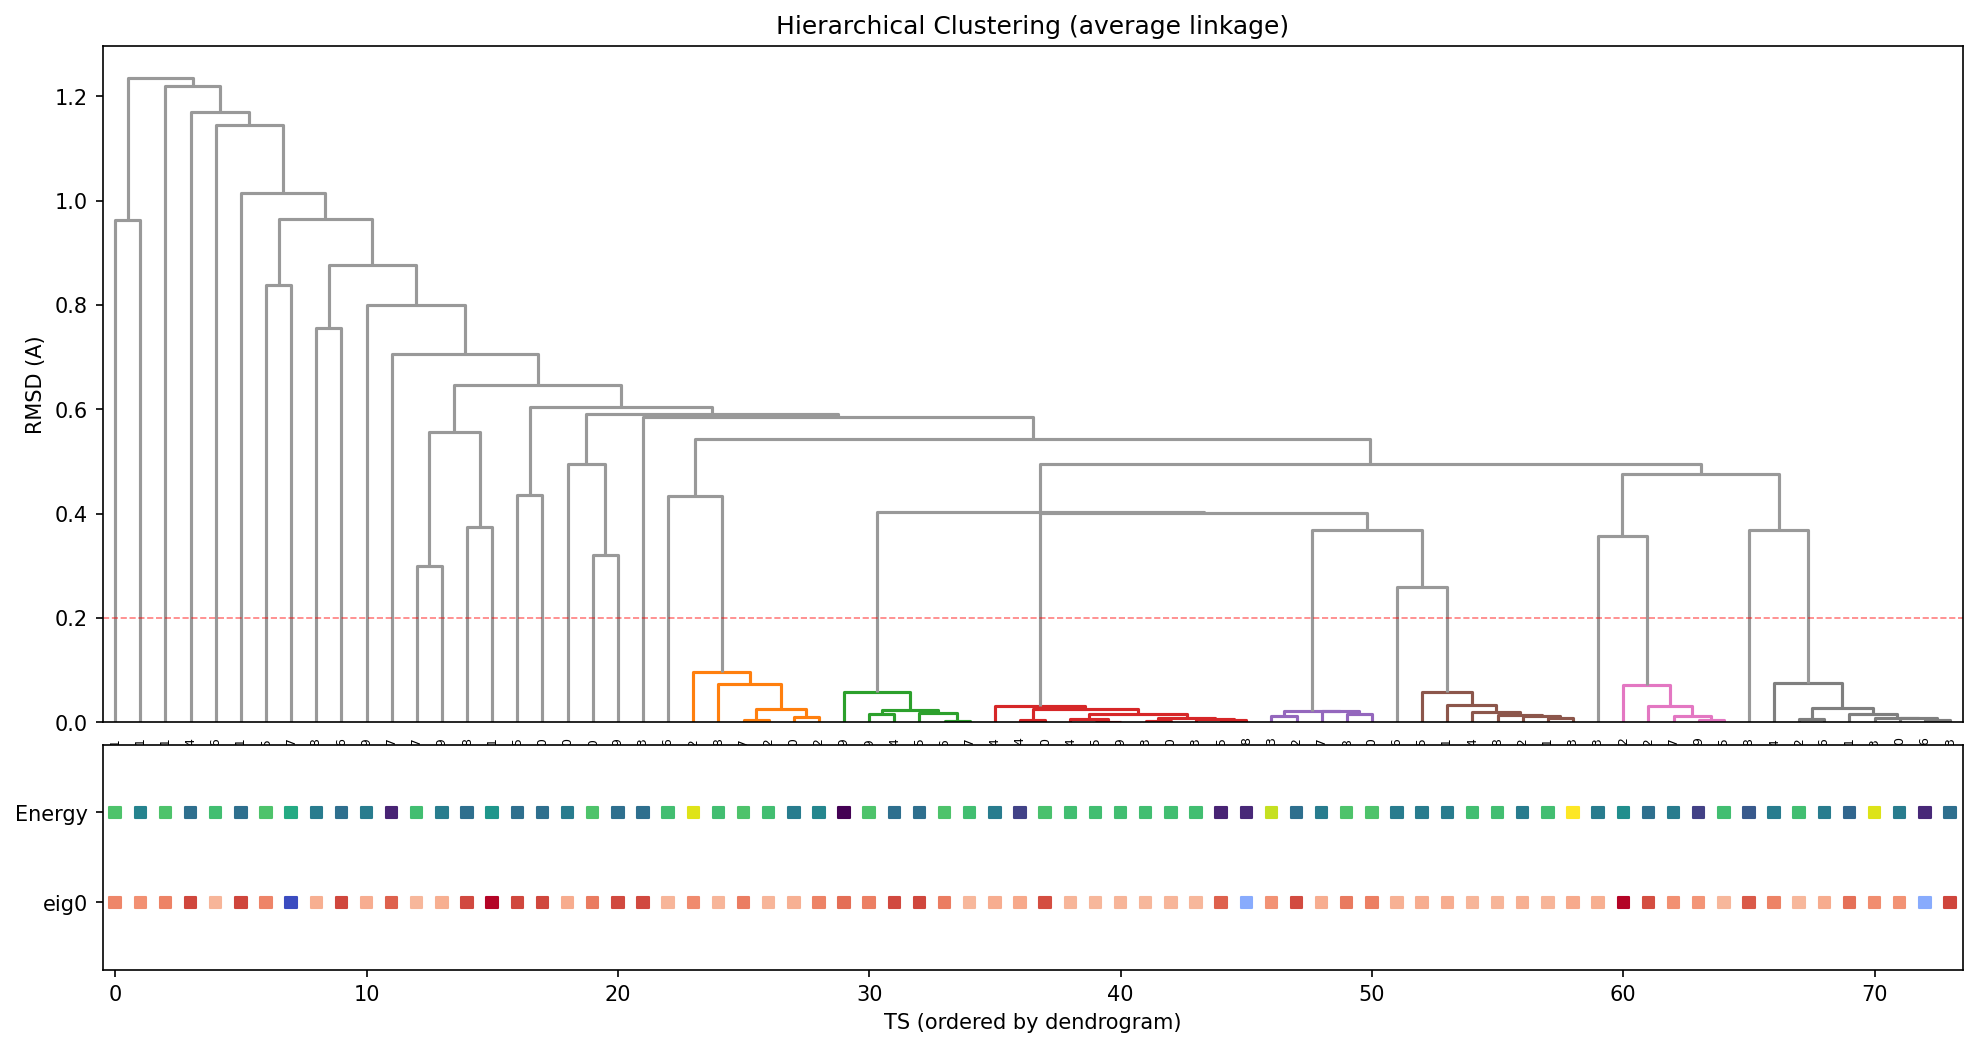
\includegraphics[width=\textwidth]{dendrogram_with_features.png}
  \caption{Hierarchical clustering dendrogram (average linkage) with energy (top color bar)
  and lowest eigenvalue (bottom color bar) mapped onto the leaf order.
  Adjacent leaves in the dendrogram often have different energy colors,
  confirming that structural proximity $\neq$ energy proximity.
  The red dashed line at 0.2~\AA{} is the original clustering threshold.}
  \label{fig:dendro}
\end{figure}

Figure~\ref{fig:dendro} visually demonstrates the RMSD--energy disconnect.
Tight structural clusters (low merge height) contain TS with different energies (different colors in the energy bar).
This is most visible in the central region ($\text{index} \sim 30$--50) where structurally similar TS
span multiple energy families.

%----------------------------------------------------------------------
\section{Embedding Visualizations}

\begin{figure}[h]
  \centering
  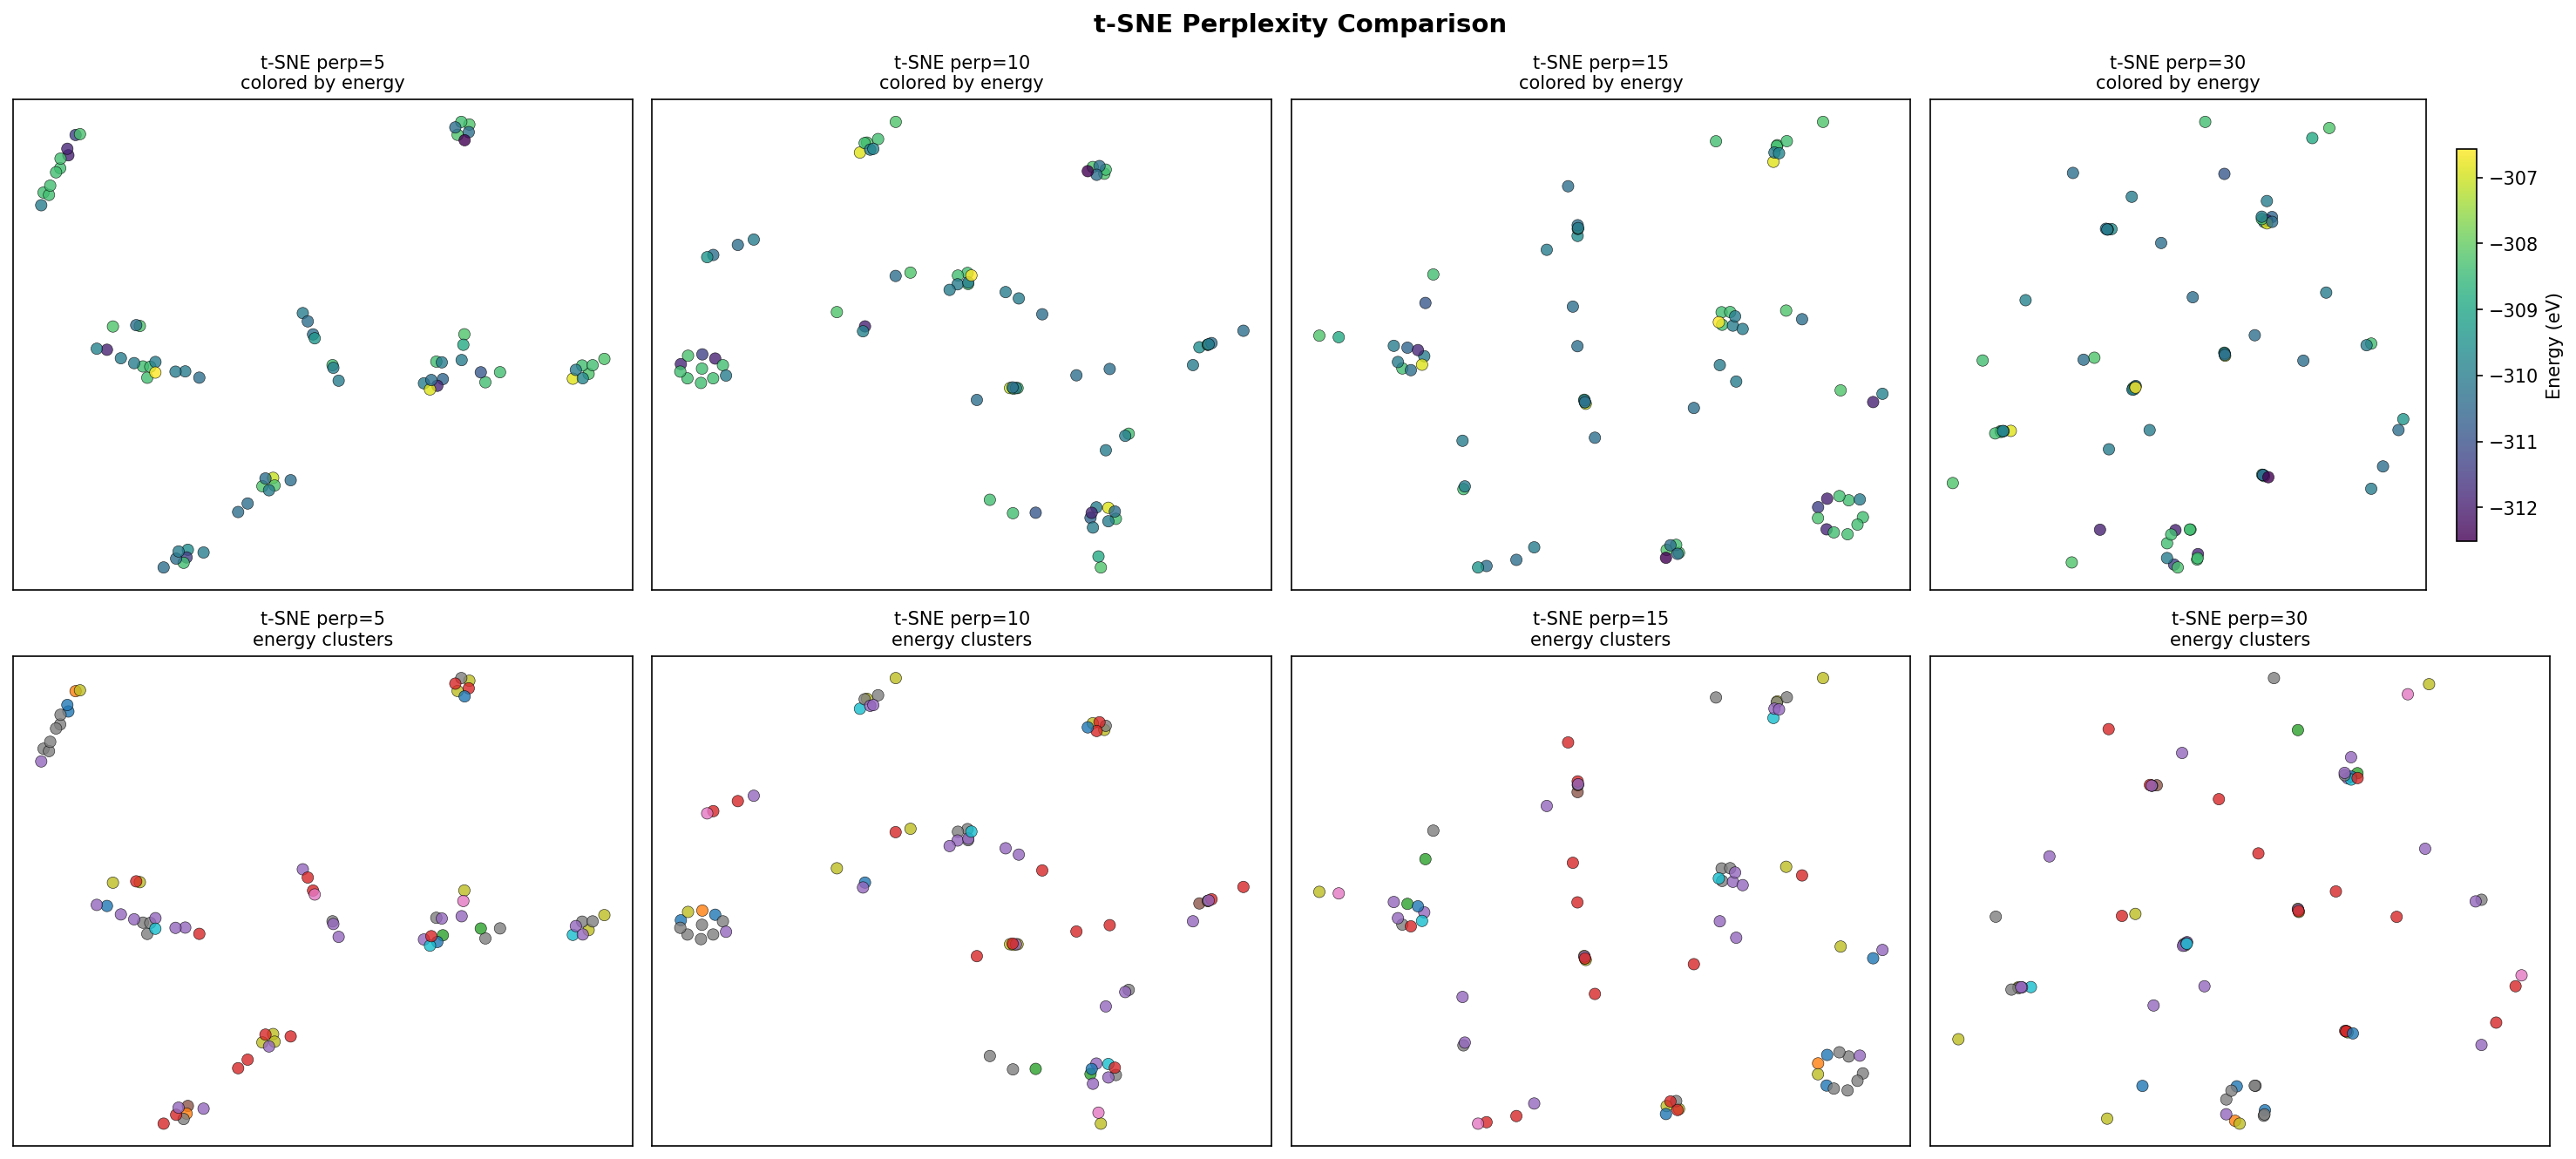
\includegraphics[width=\textwidth]{tsne_perplexity_comparison.png}
  \caption{t-SNE embeddings at perplexity 5, 10, 15, 30 (columns).
  Top: colored by energy. Bottom: colored by energy cluster assignment.
  Low perplexity (5) fragments into tight micro-clusters that mix energies.
  High perplexity (30) shows broader structure but still no clean energy separation.
  Perplexity 15 provides the best balance.}
  \label{fig:tsne}
\end{figure}

\begin{figure}[h]
  \centering
  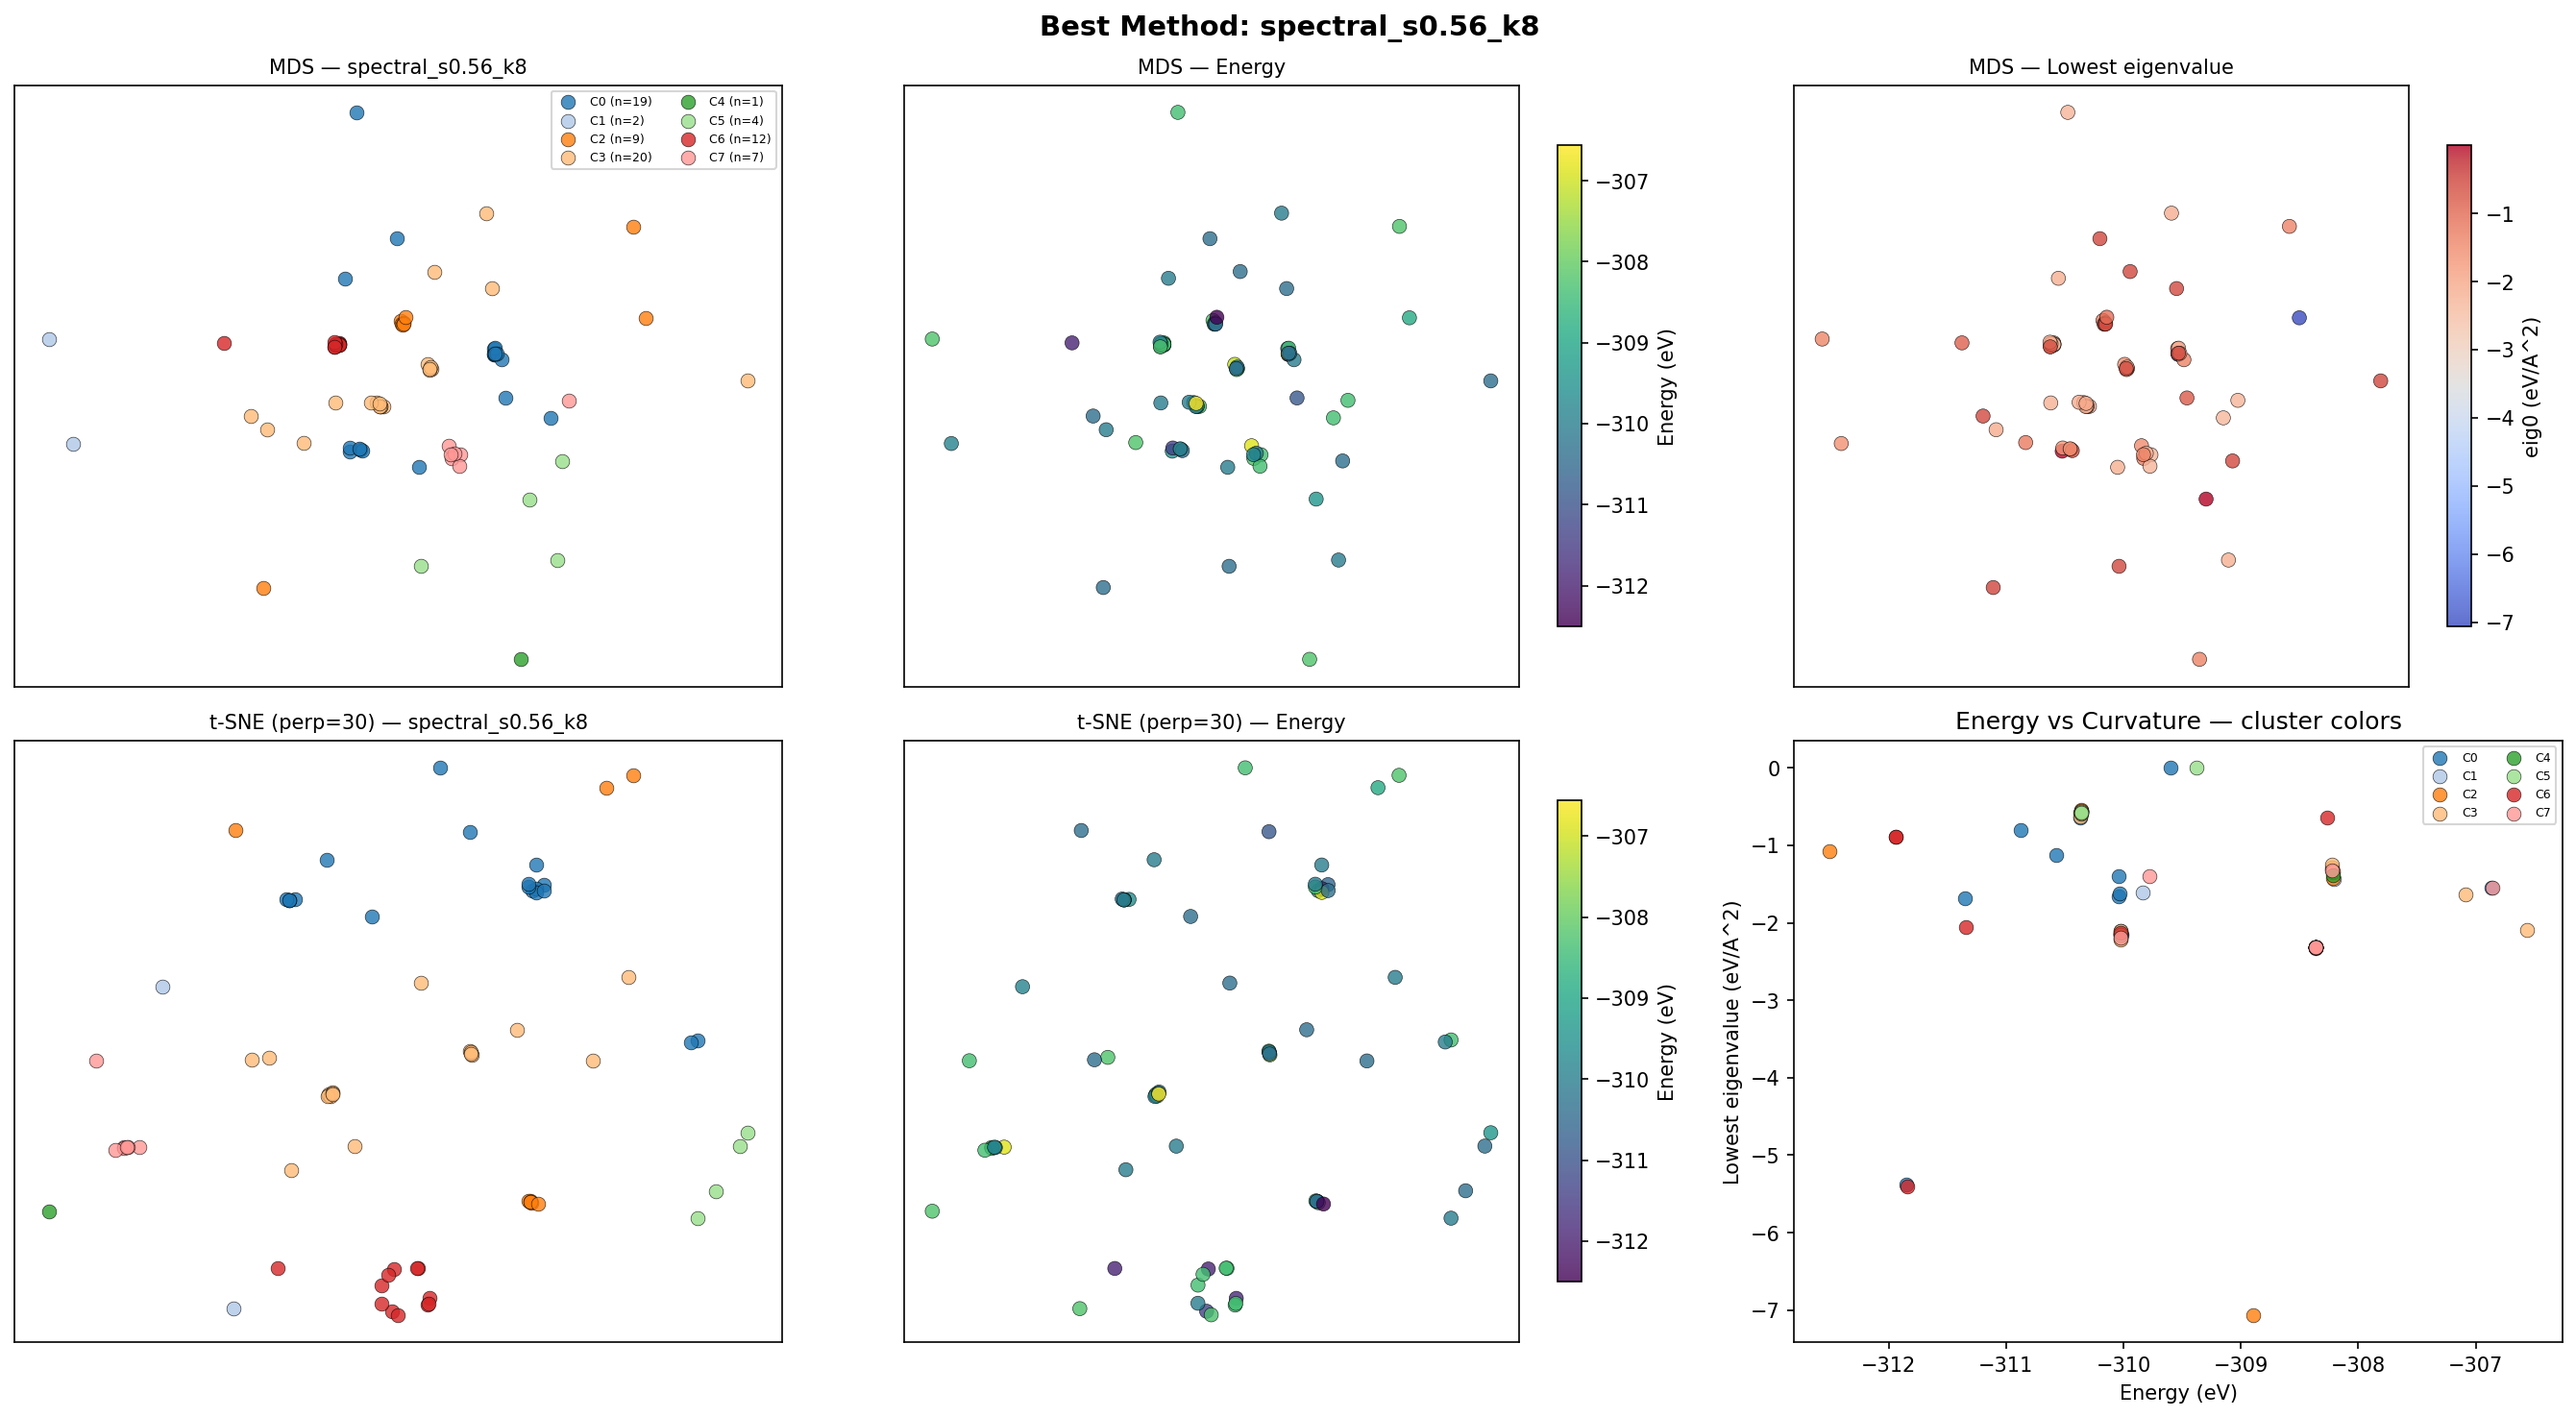
\includegraphics[width=\textwidth]{best_method_detail.png}
  \caption{The ``best'' RMSD-based method (spectral, $\sigma = 0.56$, $k = 8$; ARI $= 0.05$).
  Top row: MDS embedding colored by cluster assignment, energy, and lowest eigenvalue.
  Bottom row: t-SNE (perp$= 30$) colored by cluster and energy, plus energy vs.\ curvature scatter.
  Even the best method produces clusters that span 2+~eV in energy.}
  \label{fig:best}
\end{figure}

\begin{figure}[h]
  \centering
  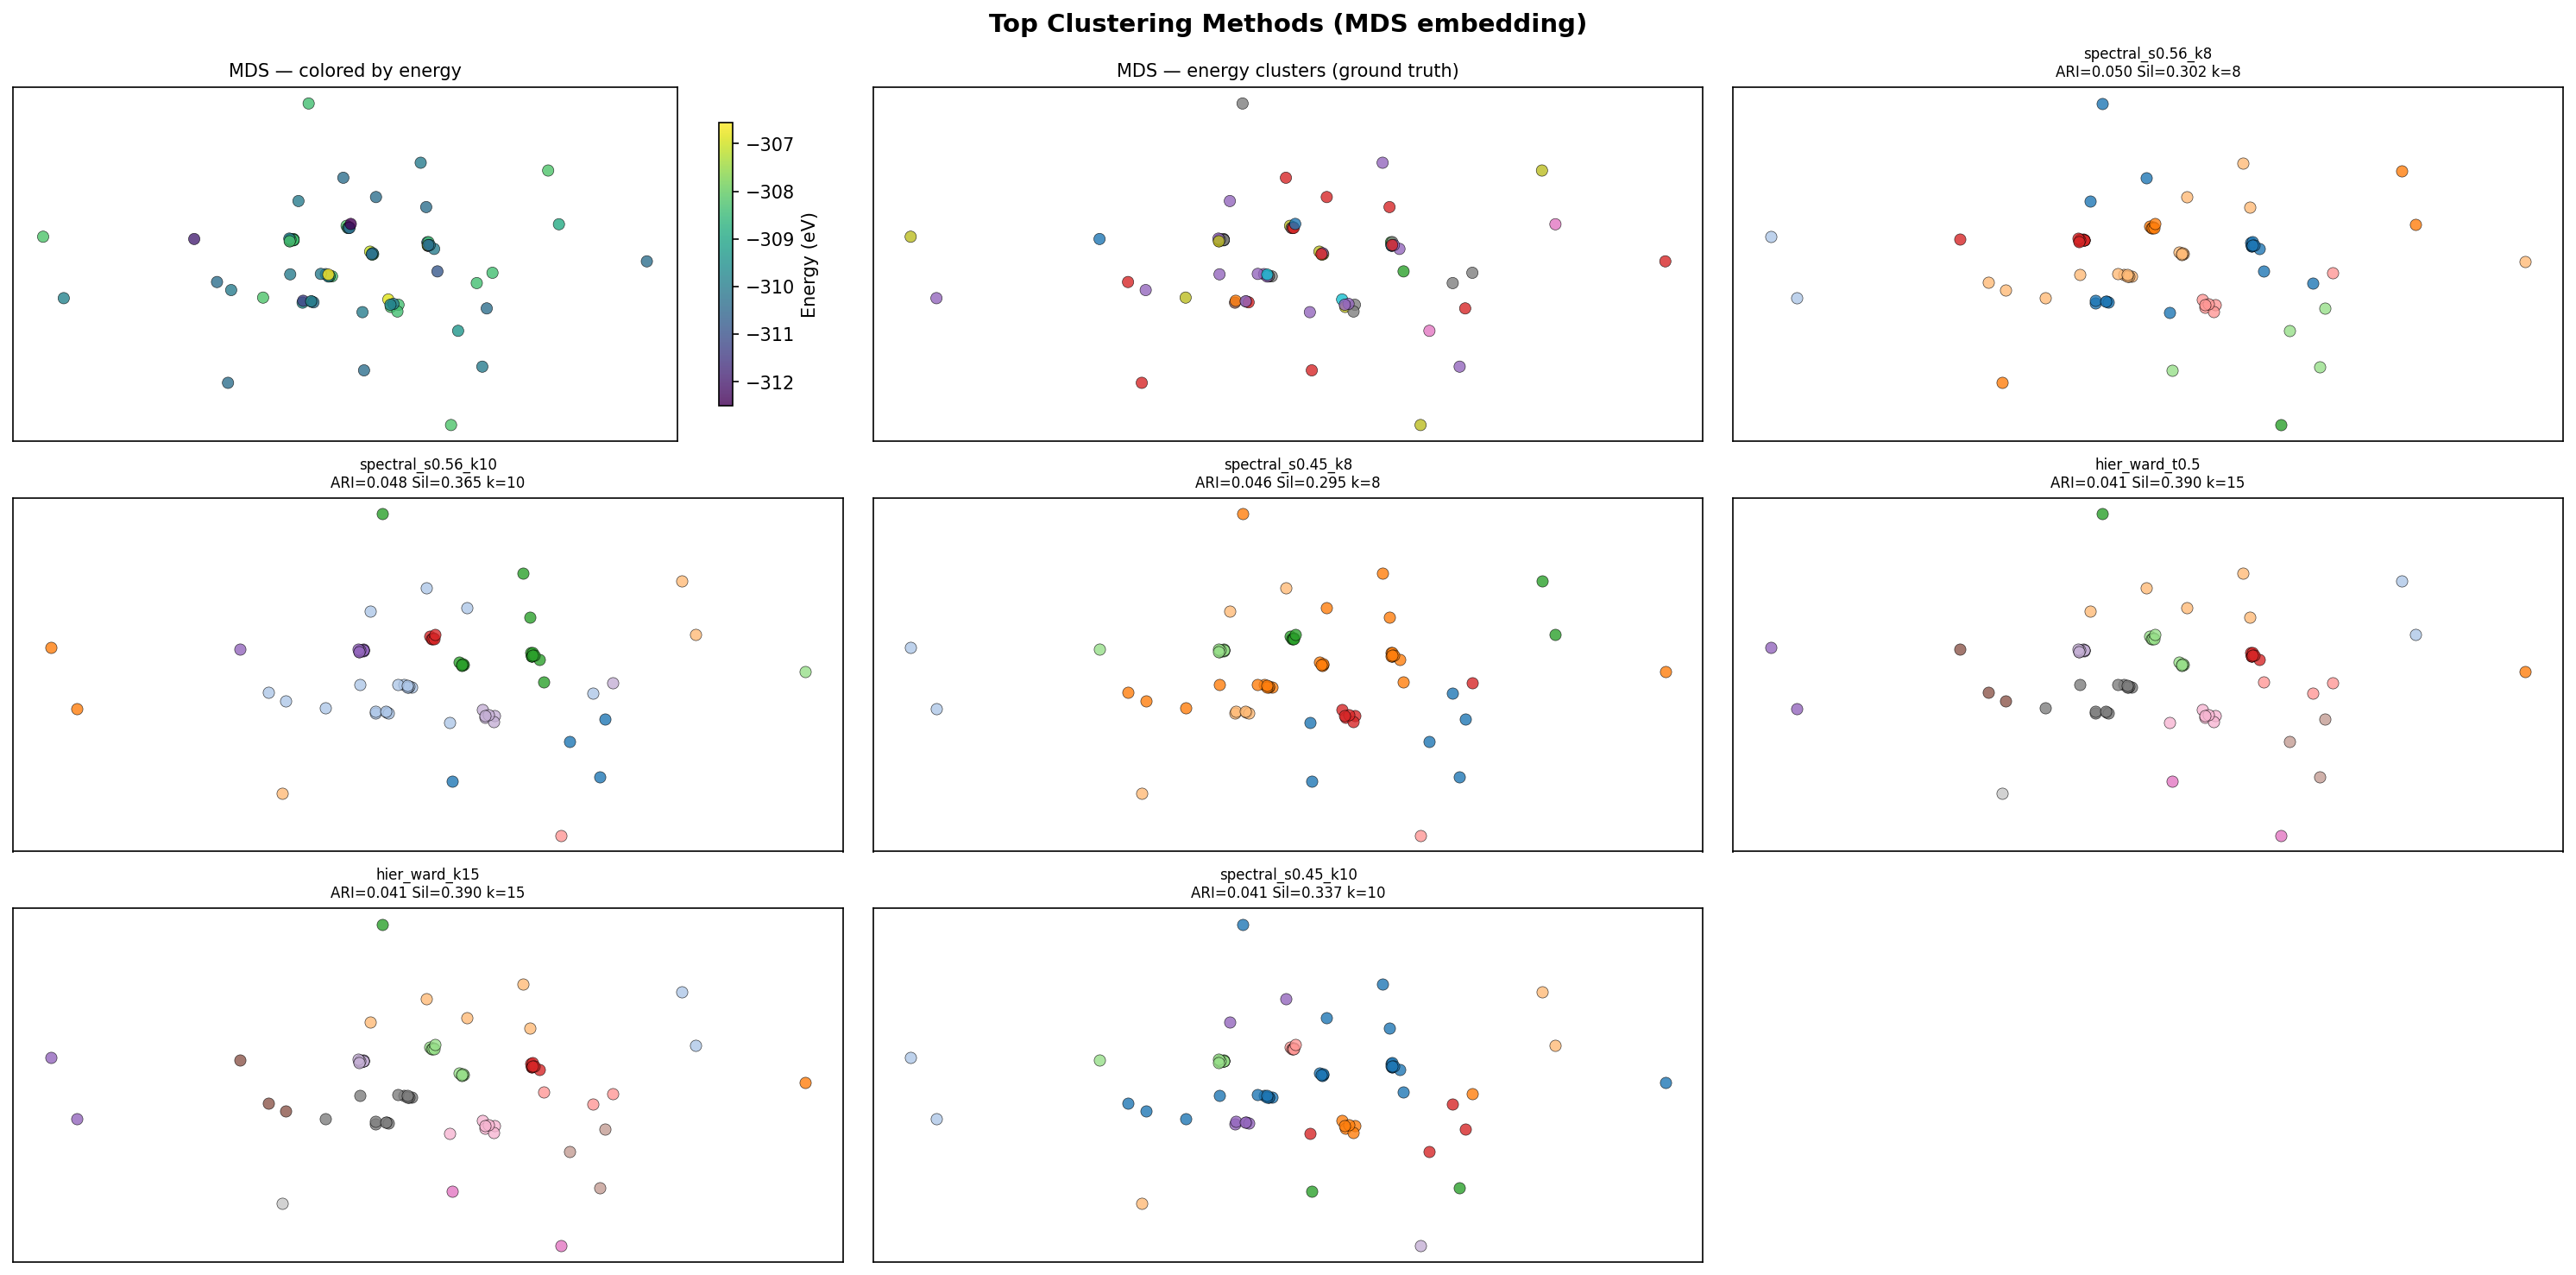
\includegraphics[width=\textwidth]{top_methods_mds_grid.png}
  \caption{MDS embedding colored by the top 6 clustering methods (ranked by ARI).
  First two panels show energy coloring and energy cluster ground truth.
  All methods produce visually different cluster assignments, and none matches the energy coloring.}
  \label{fig:grid}
\end{figure}

%----------------------------------------------------------------------
\section{Quantitative Comparison}

\begin{figure}[h]
  \centering
  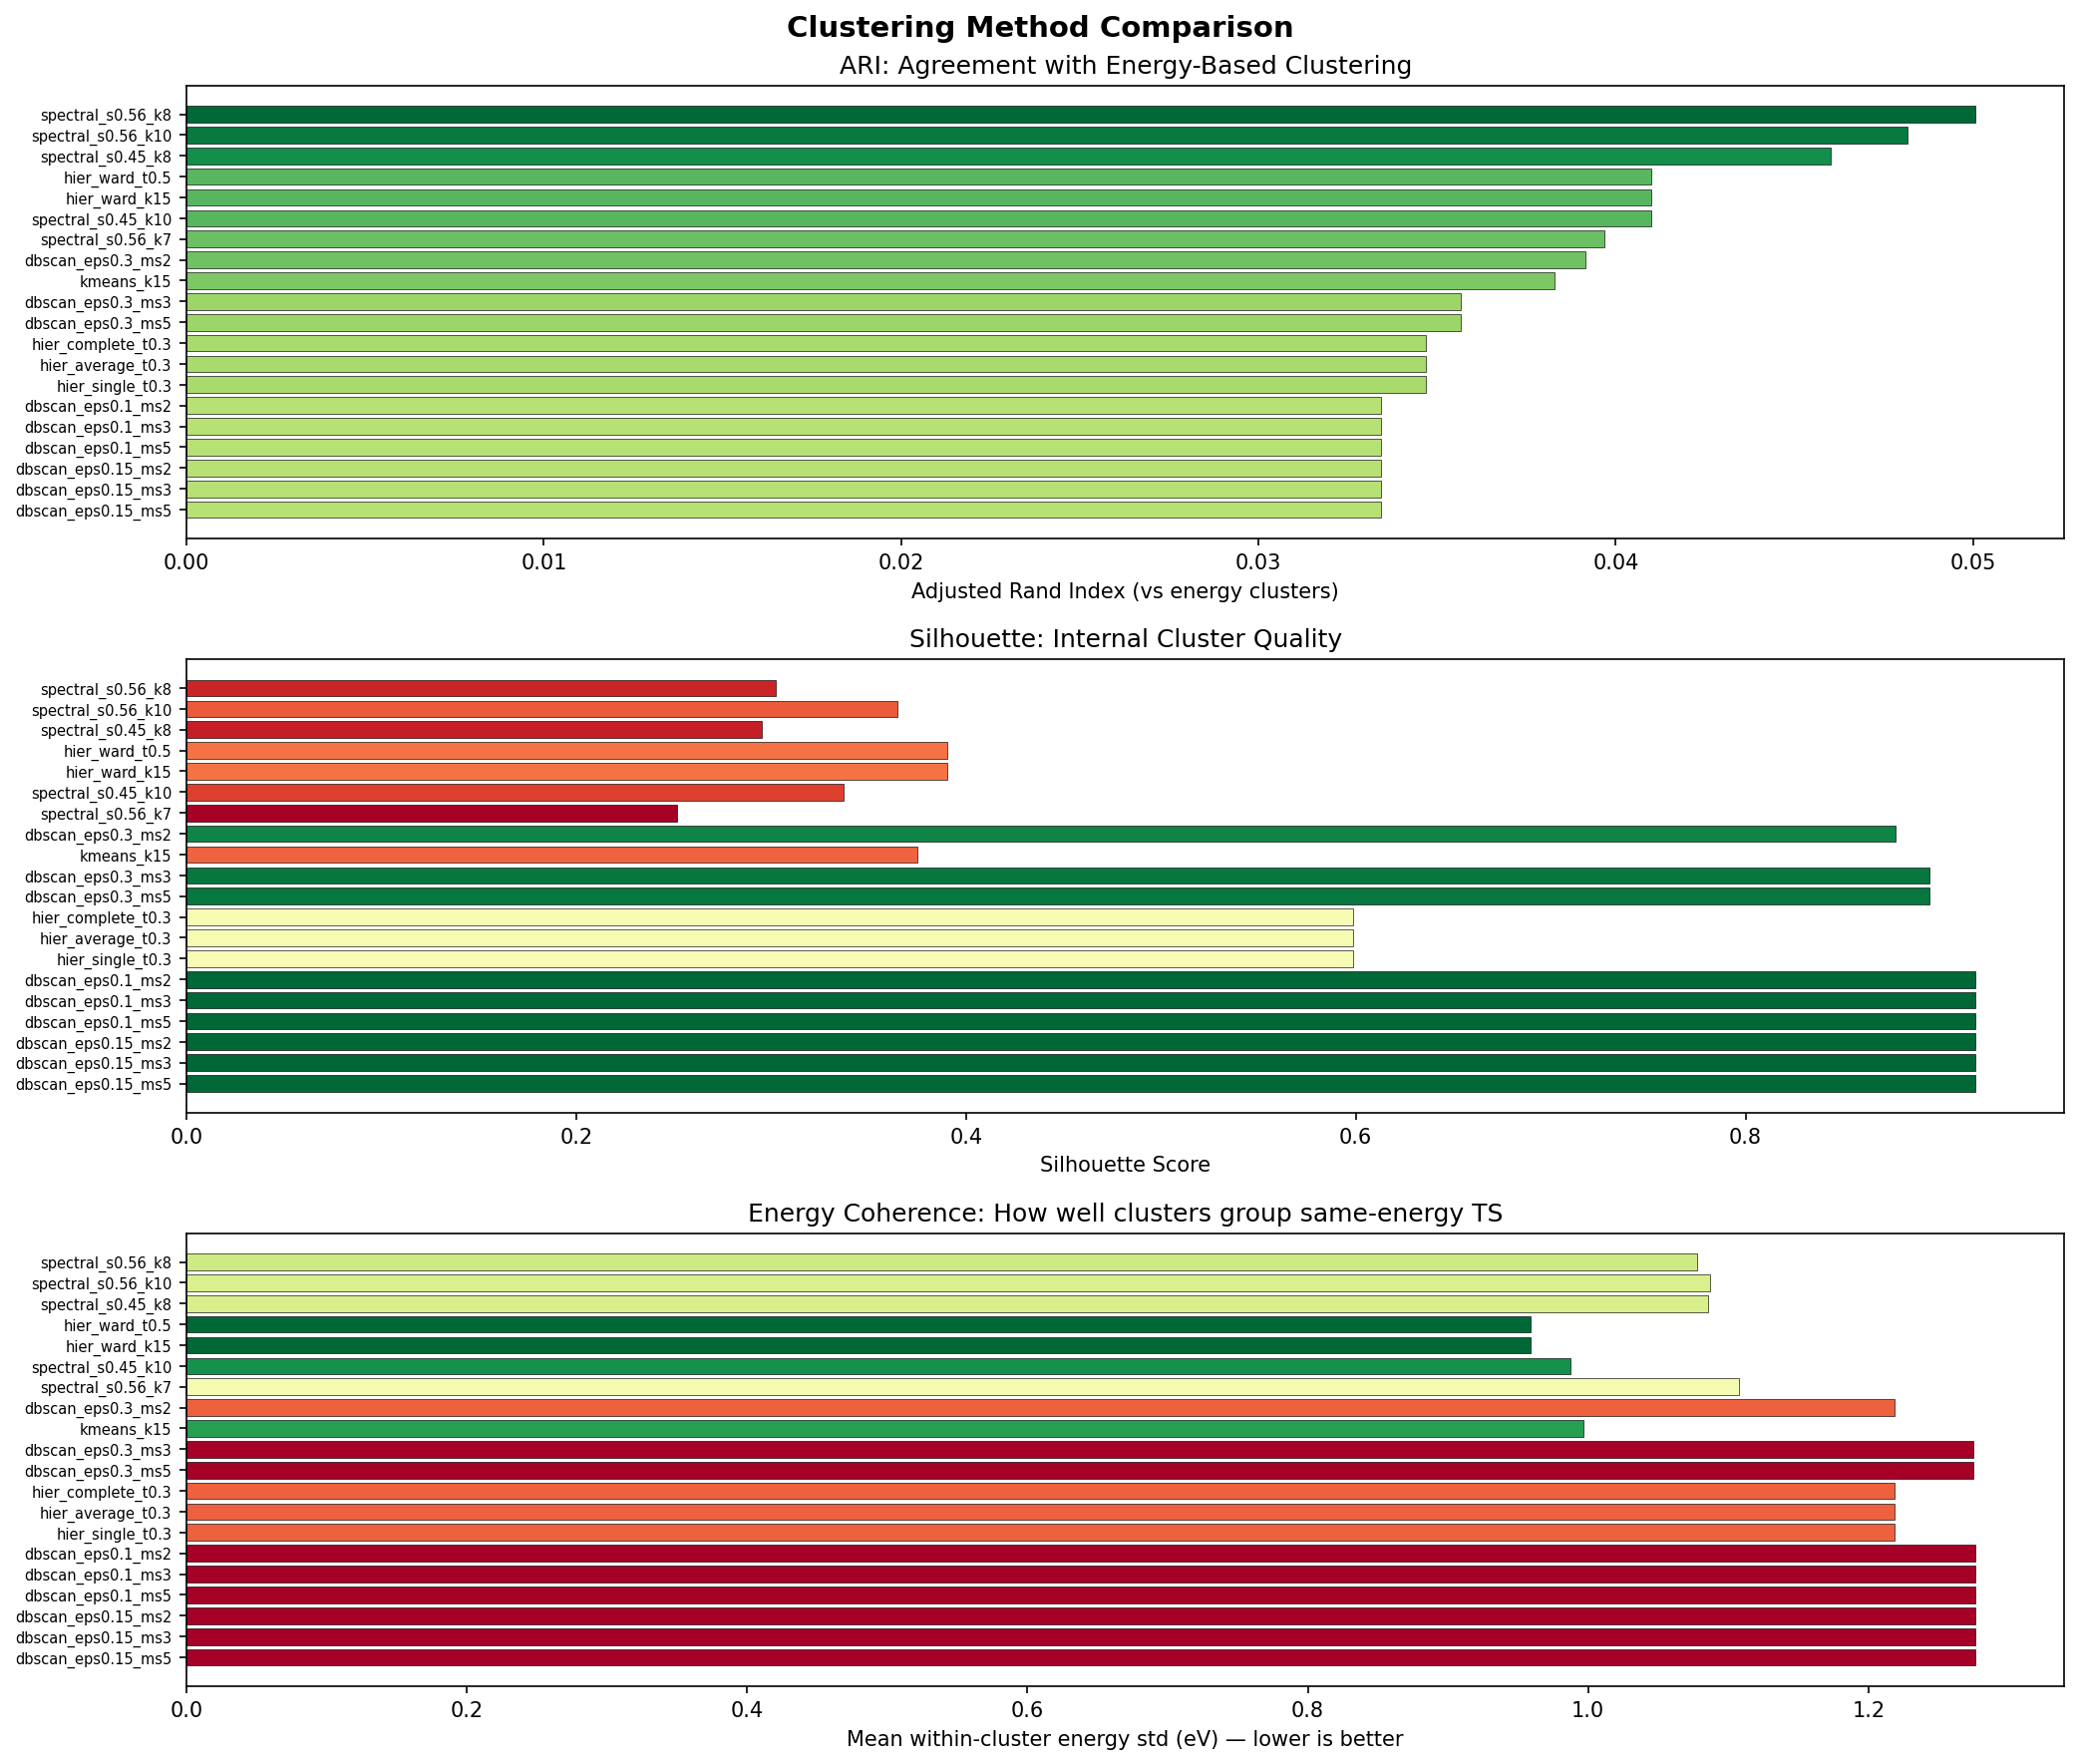
\includegraphics[width=0.85\textwidth]{metrics_comparison.png}
  \caption{Top 20 methods ranked by ARI (top), silhouette (middle), and energy coherence (bottom).
  Methods that score well on silhouette (DBSCAN, high $k$) score poorly on energy coherence,
  and vice versa. No method scores well on all three metrics simultaneously.}
  \label{fig:metrics}
\end{figure}

\begin{table}[h]
\centering
\caption{Best methods by each criterion.}
\label{tab:best}
\begin{tabular}{@{}llccc@{}}
\toprule
Criterion & Best method & $k$ & Score & Energy std (eV) \\
\midrule
ARI vs.\ energy & spectral ($\sigma{=}0.56$, $k{=}8$) & 8 & 0.050 & 1.08 \\
Silhouette & DBSCAN ($\varepsilon{=}0.05$, ms$= 2$) & 7 & 0.940 & 1.28 \\
Energy coherence & hier.\ complete ($k{=}8$) & 8 & --- & 0.70 \\
\bottomrule
\end{tabular}
\end{table}

Even the best energy-coherent method (hierarchical complete, $k = 8$) has within-cluster energy
standard deviation of 0.70~eV, which is large given the 6~eV energy range.

%----------------------------------------------------------------------
\section{Conclusions}

\begin{enumerate}
  \item \textbf{RMSD clustering $\neq$ energy clustering.} All 131 RMSD-based methods achieve ARI $< 0.05$
    against energy-based ground truth. Structural similarity and chemical identity are decoupled for
    isopropanol TS on DFTB0.

  \item \textbf{No natural structural cluster count.} Silhouette analysis shows no elbow; DBSCAN
    robustly finds 7 tight clusters but classifies 30/74 TS as noise.

  \item \textbf{Methods agree within families, not across.} Hierarchical methods agree with each other
    (ARI $\sim 0.3$--1.0), but not with DBSCAN or spectral (ARI $< 0.2$).

  \item \textbf{For diffusion model training}, TS should be classified by energy (or energy + eigenvalue),
    not by RMSD. The 5 main energy families (A--E) are the chemically meaningful grouping.

  \item \textbf{RMSD clustering is still useful} for identifying structural sub-variants (H-rotamers,
    mirror images) \emph{within} an energy family, but not for distinguishing families.
\end{enumerate}

\end{document}
